\documentclass[12pt,a4]{article}

\usepackage{inputenc}
\usepackage[T1]{fontenc}
\usepackage{amsmath,amsfonts,amsthm}
\usepackage{graphicx}

\newcommand{\R}{{\mathbb R}}
\newcommand{\C}{{\mathbb C}}
\newcommand{\N}{{\mathbb N}}
\newcommand{\ra}{\rightarrow}
\newcommand{\eps}{\varepsilon}

\newtheorem{theorem}{Theorem}



\title{Inversion of the Laplace transform}
\author{Lasse Lybeck\\013748498}


\begin{document}

\maketitle

\section{Introduction}

Let $f:[0,\infty)\rightarrow \R$. The Laplace transform $F$ of $f$ is defined by
\begin{equation}\label{laplace}
 F(s) = \int_0^\infty e^{-st}f(t)dt,\quad s\in\C ,
\end{equation}
provided that the integral converges.

The transform has many applications in physical sciences and is therefore widely used and studied. One example of the usage of the transform is in linear differential equations, which may in some cases be easily solved using the Laplace transform.

The direct problem is to determine $F$ for a given function $f$ according to (\ref{laplace}). The inverse problem is: {\em given a Laplace transform $F$, find the corresponding function $f$.} In this study we will be looking at the inverse problem from the computational point of view. We will notice that the inverse problem is ill-posed and not at all trivial.




\section{Materials and Methods}\label{sec:methods}

\subsection{Theoretical basis}

In this study we will solve the inverse problem with the \emph{truncated singular value decomposition} method. In the future we will refer to the singular value decomposition as SVD. Let us first revise the theory for the SVD and the pseudoinverse.

\subsubsection{Singular value decomposition and the pseudoinverse}

The truncated SVD method is based on the fact that every matrix $A \in \R^{m \times n}$ can be decomposed into the product of three matrices
\begin{equation}
A = U D V^T,
\end{equation}
where $U$ and $V$ are orthogonal matrices and $D$ is a diagonal matrix. The diagonal elements $d_{i,i}$, $i = 1, \ldots , min \left\{ m,n \right\}$ of $D$ are called the \emph{singular values of $D$}.

The \emph{pseudoinverse} of $A$ (denoted as $A^+$) can be calculated via the SVD of $A$. Due to the fact that $U$ and $V$ are orthogonal, we know that $U^T = U^{-1}$ and $V^T = V^{-1}$. We define the pseudoinverse of the diagonal matrix $D \in \R^{m \times n}$ as the diagonal matrix $D^+ \in \R^{n \times m}$ where the diagonal elements have the values
\begin{equation}
D^+_{i,i} =
\begin{cases}
    1 / d_{i,i} & \text{if }d_{i,i} \neq 0 \\
    0           & \text{otherwise}.
\end{cases}
\end{equation}
Now we can define the pseudoinverse of $A$ as 
\begin{equation}\label{pseudo}
A^+ = V D^+ U^T .
\end{equation}

If $A \in \R^{n \times n}$ is invertible we notice that $A^+ = A^{-1}$. As it is easily shown that $D D^+ = D^+ D = I$ we get
\begin{equation}
A A^+ = U D \underbrace{V^T V}_{= I}  D^+ U = U \underbrace{D D^+}_{= I} U^T = U U^T = I
\end{equation}
and in a similar manner
\begin{equation}
A^+ A = V D^+ U^T U D V^T = V D^+ D V = V V^T = I ,
\end{equation}
and thus we see that $A^+ = A^{-1}$. This is however often not the case.

In the case of linear systems $Af = m$ we get the least squares solution easily with the pseudo inverse of $A$. The following result is shown in the work \cite{samu}, and we will not be proving it here. Notice that in the case of the following theorem $A$ need not be invertible, for example if $A \in \R^{m \times n}$, where $m > n$.

\begin{theorem}
Let $A \in \R^{m \times n}$. The minimum norm solution of the linear system $Af = m$ is given by $A^+ m$.
\end{theorem}
\begin{proof}
See \cite{samu} theorem 4.1.
\end{proof}


\subsubsection{Truncated singular value decomposition}

Although we have shown that linear systems $Af = m$ can easily be solved with the pseudoinverse of the coefficient matrix $A$, this will not always be the proper way of solving inverse problems of the same type.

\subsection{The matrix model}\label{sec:matrixmodel}

Assume we know the values of $F$ at these real-valued points:
$$
 0<s_1<s_2<\ldots <s_n<\infty.
$$ 
Then we may approximate the integral in (\ref{laplace}) for example with the trapezoidal rule as
\begin{equation} \label{laptrap}
\begin{split}
 \int_0^\infty e^{-st}f(t)dt\, \approx\, \frac{t_k}{k} & \left( \frac{1}{2}e^{-st_1}f(t_1)+e^{-st_2}f(t_2)+e^{-st_3}f(t_3)+\ldots\right.\\   &\ \ \left. +e^{-st_{k-1}}f(t_{k-1})+\frac{1}{2}e^{-st_k}f(t_k)\right) ,
\end{split}
\end{equation}
where vector $t=[t_1\ t_2\ \ldots\ t_k]^T\in\R^k$, $0\leq t_1<t_2<\ldots <t_k$, contains the points at which the unknown function $f$ will be evaluated. By denoting $f_\ell=f(t_\ell), \ \ell=1,\ldots ,k$, and $m_j=F(s_j),\ j=1,\ldots ,n$, and using \eqref{laptrap}, we get a linear model of the form $m=Af+\epsilon$ with
\begin{equation}\label{LaplaceA} 
A = \frac{t_k}{k}\begin{bmatrix} \frac{1}{2}e^{-s_1t_1} & e^{-s_1t_2} & e^{-s_1t_3} & \ldots & e^{-s_1t_{k-1}} & \frac{1}{2}e^{-s_1t_k} \\
                       \frac{1}{2}e^{-s_2t_1} & e^{-s_2t_2} & e^{-s_2t_3} & \ldots & e^{-s_2t_{k-1}} & \frac{1}{2}e^{-s_2t_k} \\
                       \vdots & & & & & \vdots \\
                       \frac{1}{2}e^{-s_nt_1} & e^{-s_nt_2} & e^{-s_nt_3} & \ldots & e^{-s_nt_{k-1}} & \frac{1}{2}e^{-s_nt_k} \end{bmatrix}.
\end{equation}


\subsection{The inversion method}

As the materials for this study we have created MATLAB code for calculating the inverse Laplace transform with the truncated SVD method. The starting point for out experiments is as follows.

The measurements were done with the function $f: \left[ 0, \infty \right[ \ra \R$,
\begin{equation}\label{eq:f}
f(t) = 
\begin{cases}
1, & \text{for } 0 \leq t \leq 1 \\
0, & \text{otherwise}.
\end{cases}
\end{equation}

The matrix $A$ and vectors $s$ and $t$ are defined as explained in section \ref{sec:matrixmodel}. The values of $s_i$ of the vector $s \in \R^n$ and $t_j$ of the vector $t \in \R^k$ were chosen evenly spaced from the intervals $\left] 0, 100 \right[$ and $\left[ 0,3 \right]$, respectively. The values of $n$ and $k$ were varied in the experiments to determine their effect on the results.

With the specified function $f$ the Laplace transform can be calculated as
\begin{equation}
F(s) = \int_0^{\infty} e^{-st} f(t) dt
     = \int_0^1 e^{-st} dt
     = \frac{1 - e^{-s}}{s},
\end{equation}
and thus the values of the Laplace transform can be easily without using numerical integration methods. This adds both speed and precision to the calculations.

We then created the measurement points $m = [m_1, m_2, \ldots, m_n]^T + \eps$, where $m_i = F(s_i)$, $F$ is defined as in \eqref{laplace} for the function $f$ and $\eps$ is some random noise.

The reconstruction $T_\alpha(m)$ from the measurement data $m$ of the function $f$ in the interval $\left[0,3\right]$ could then be calculated with the truncated SVD method with $\alpha$ as the regularization parameter. The results were then recorded with different choices of $\alpha$.



\section{Results}\label{sec:results}

\begin{figure}[t]
\begin{center}
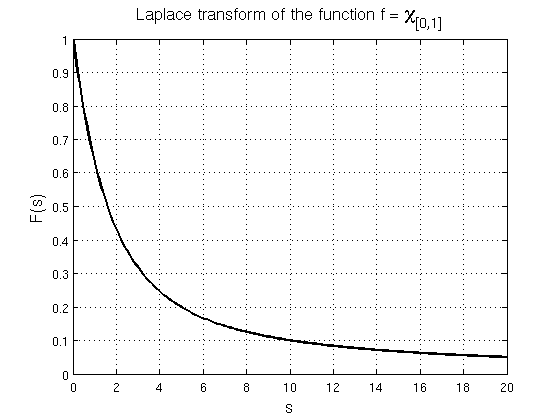
\includegraphics[scale=.6]{img/laplace.png}
\end{center}
\caption{Laplace transform of $f$}
\label{fig:laplace}
\end{figure}

\begin{figure}[t]
\begin{center}
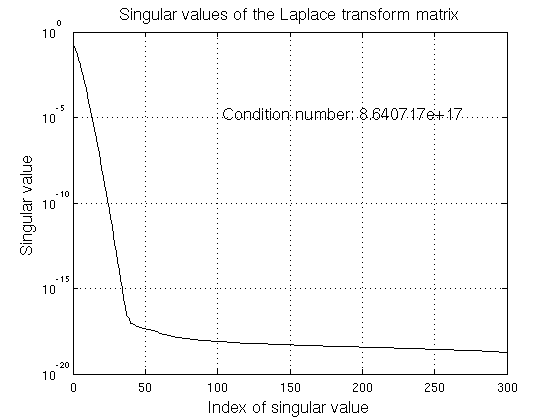
\includegraphics[scale=.6]{img/singular.png}
\end{center}
\caption{Singular values of a Laplace transform matrix}
\label{fig:singular}
\end{figure}

\begin{figure}[t]
\begin{center}
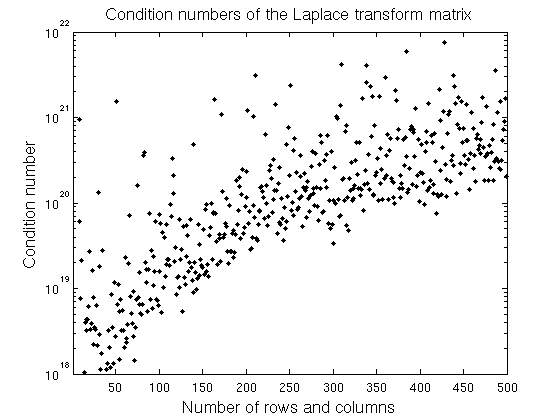
\includegraphics[scale=.6]{img/cond.png}
\end{center}
\caption{Condition numbers of $k \times k$ Laplace transform matrices}
\label{fig:cond}
\end{figure}

The Laplace transform of the function $f$ defined in \eqref{eq:f} is shown in figure \ref{fig:laplace}. The measurement data used in the inversion of the Laplace transform will be similar to what is seen in the figure, but with added noise and on a wider interval.

In figure \ref{fig:singular} the singular values are shown for a certain Laplace transform matrix $A$. The matrix is constructed with the vectors $t \in \R^k$ and $s \in \R^n$, with the values $k = 1000$ and $n = 300$. The condition number for the matrix is, as shown in the figure, about
\begin{equation}
\text{cond}(A) \approx 8.6407 \cdot 10^{17}.
\end{equation}





\section{Discussion}

\subsection{Ill-posedness}

As it can be seen from figure \ref{fig:singular}, the singular values of the coefficient matrix are decreasing very rapidly (notice the logarithmic scale on the y-axis). This results in high condition numbers and therefore in systems with high sensibility for noise. As it can further be seen from figure \ref{fig:cond}, the condition number greatly increases as the size of the matrix increases (again, notice the logarithmic scale). These results clearly point to the fact that the inverse Laplace transform is an ill-posed problem.


\newpage
\begin{thebibliography}{9}

\bibitem{samu}
Mueller, Jennifer L., ; Siltanen, Samuli \\
\emph{Linear and nonlinear inverse problems with practical applications} \\ Philadelphia : SIAM, 2012. - (Computational science \& engineering.)

\end{thebibliography}

\end{document}



